\chapter{Processes, Threads, and Scheduling}
\label{chap:processes}

In any multitasking operating system, the most central abstraction is the \textbf{process}. A process is simply an executing program along with all the state required to run it: its virtual address space, CPU register values, thread stacks, file descriptor tables, IPC channels, and security credentials.

Tanenbaum famously compared a computer running multiple processes to a busy chef baking cakes~\cite{tanenbaum2006operating}: the chef (the CPU) switches rapidly between distinct recipes (the programs) and their respective bowls of ingredients (the address spaces). To the outside observer, multiple cakes appear to be rising simultaneously.

In this chapter, we explore how modern operating systems structure processes and threads, examine the mathematical and algorithmic foundations of CPU scheduling, dive into mutual exclusion and synchronization primitives (from hardware atomic instructions to Linux-compatible futexes), and dissect the implementation of Hydra's preemptive scheduler and context switch engine.

% ==============================================================================
\section{The Process Model}
\label{sec:process_model}
% ==============================================================================

In modern operating systems, all runnable software is organized into one or more sequential processes. A process is an independent execution entity consisting of:
\begin{enumerate}
    \item \textbf{A Private Virtual Address Space:} Mapped via hardware page tables, ensuring that the process can read and write only its own memory cells.
    \item \textbf{A Thread of Execution:} A sequential stream of instructions guided by a Program Counter (the \texttt{RIP} register on x86\_64) and executed in the context of processor registers and a stack.
    \item \textbf{Kernel-Managed Resources:} File descriptor tables, capability rights tokens, signal masks, parent-child relationships, and memory-mapped files.
\end{enumerate}

\subsection{Process Creation and Lifecycle}
Operating systems create processes in four primary situations:
\begin{enumerate}
    \item \textbf{System Initialization:} When the kernel boots, it initializes hardware subsystems and creates root processes (such as the Hydra shell, the idle task, and the supervisor).
    \item \textbf{Execution of a Process Creation System Call:} An actively running process invokes a system call (such as \texttt{fork()}, \texttt{clone()}, or \texttt{posix\_spawn()}) to launch a subsidiary process.
    \item \textbf{User Request:} An interactive user types a command into the shell or double-clicks an application icon in a graphical desktop environment (e.g., KDE Plasma).
    \item \textbf{Batch Job Initiation:} A job scheduler (such as cron or a compute cluster manager) activates a queued batch job.
\end{enumerate}

In UNIX and modern POSIX-compliant systems, process creation is classically split into two complementary system calls:
\begin{itemize}
    \item \texttt{fork()}: Creates an exact duplicate of the calling process, including an identical copy of the virtual address space (implemented with high efficiency using Copy-on-Write page table manipulation).
    \item \texttt{execve()}: Replaces the calling process's current memory image, code segment, and heap with a new binary executable file read from disk (such as an ELF binary), resetting registers and commencing execution at the new entry point.
\end{itemize}

\subsection{Process Termination}
A process terminates under one of four conditions:
\begin{enumerate}
    \item \textbf{Normal Exit (Voluntary):} The process completes its task and invokes \texttt{exit(0)} (system call \texttt{sys\_exit}).
    \item \textbf{Error Exit (Voluntary):} The process encounters a fatal logic error (e.g., a compiler fails to open an input source file) and invokes \texttt{exit(status)} with a non-zero exit code.
    \item \textbf{Fatal Error (Involuntary):} The process triggers an unhandled CPU exception (e.g., dividing by zero, dereferencing an unmapped memory address triggering a Page Fault \texttt{\#PF}, or executing an illegal instruction triggering an Invalid Opcode \texttt{\#UD}). The kernel terminates the process, optionally generating a core dump file.
    \item \textbf{Killed by Another Process (Involuntary):} Another authorized process or the operating system sends a terminating signal (e.g., \texttt{SIGKILL} or \texttt{SIGTERM}) via the \texttt{kill()} system call.
\end{enumerate}

\subsection{Process Hierarchies and State Transitions}
In Hydra, as in UNIX, processes are organized into a strict hierarchical tree rooted at the initial supervisor process (\texttt{PID~1}). When a parent process spawns a child, the parent remains responsible for reaping the child when it terminates.

A process transitions through distinct states during its lifespan, as illustrated in Figure~\ref{fig:process_states}:
\begin{itemize}
    \item \textbf{Running:} The process is actively executing machine instructions on a CPU core.
    \item \textbf{Ready:} The process is fully prepared to execute, but is temporarily suspended waiting for the scheduler to allocate it a CPU time slice.
    \item \textbf{Blocked:} The process cannot execute because it is waiting for an external event (e.g., disk I/O completion, an incoming network packet, or a synchronous IPC rendezvous). Even if a CPU core were free, the process cannot run.
    \item \textbf{Sleeping:} A specialized blocked state in which the process is paused until a target timer tick is reached (e.g., via \texttt{nanosleep()}).
    \item \textbf{Dead / Zombie:} The process has terminated execution. Its memory and file descriptors have been released, but its \texttt{TaskControlBlock} remains in the process table so that its parent can inspect its final exit status code via \texttt{waitpid()}. Once reaped, the entry is deleted.
\end{itemize}

\begin{figure}[htbp]
\centering
\begin{tikzpicture}[scale=0.9, every node/.style={transform shape}]
    \node[draw=hydrablue, fill=hydralight, rounded corners, minimum width=2.5cm, minimum height=1.2cm, font=\bfseries\sffamily] (ready) at (0, 0) {Ready};
    \node[draw=rustred, fill=rustred!15, rounded corners, minimum width=2.5cm, minimum height=1.2cm, font=\bfseries\sffamily] (running) at (5, 0) {Running};
    \node[draw=hydragold, fill=hydragold!20, rounded corners, minimum width=2.5cm, minimum height=1.2cm, font=\bfseries\sffamily] (blocked) at (2.5, -3) {Blocked / Sleeping};
    \node[draw=black, fill=gray!20, rounded corners, minimum width=2.5cm, minimum height=1.2cm, font=\bfseries\sffamily] (dead) at (10, 0) {Dead / Zombie};

    \draw[->, >=Stealth, line width=1.2pt, hydrablue] (ready) to[bend left=20] node[above] {\small Scheduler Dispatch} (running);
    \draw[->, >=Stealth, line width=1.2pt, rustred] (running) to[bend left=20] node[below] {\small Timeslice Expired} (ready);
    \draw[->, >=Stealth, line width=1.2pt, hydragray] (running) to[bend left=20] node[right] {\small Wait for I/O / IPC} (blocked);
    \draw[->, >=Stealth, line width=1.2pt, hydragold] (blocked) to[bend left=20] node[left] {\small Event Occurs / Wakeup} (ready);
    \draw[->, >=Stealth, line width=1.2pt, black] (running) -- node[above] {\small \texttt{sys\_exit()}} (dead);
\end{tikzpicture}
\caption{The Process State Transition Diagram in Hydra.}
\label{fig:process_states}
\end{figure}

% ==============================================================================
\section{The Thread Model and Multithreading}
\label{sec:thread_model}
% ==============================================================================

In traditional operating systems, each process possessed a single thread of control. However, modern software systems perform multiple concurrent activities within the same application:
\begin{itemize}
    \item A web browser must concurrently render HTML elements, execute JavaScript animations, stream video, and download incoming TCP packets over multiple connections.
    \item A database server must service hundreds of concurrent client queries while background threads flush write-ahead transaction logs to disk.
\end{itemize}

\subsection{Threads versus Processes}
A \textbf{thread} (or lightweight process) is an independent execution context that shares an address space and open file descriptors with other threads in the same process:

\begin{table}[htbp]
\centering
\small
\begin{tabular}{ll}
\hline
\textbf{Per-Process Items (Shared by all Threads)} & \textbf{Per-Thread Items (Private to each Thread)} \\
\hline
Virtual Address Space (PML4 page tables) & Program Counter (\texttt{RIP}) \\
Executable Machine Code & CPU Register Set (\texttt{RAX}, \texttt{RBX}, etc.) \\
Global Variables and Static Data & Execution Stack (Stack Pointer \texttt{RSP}) \\
Heap Allocations & Thread-Local Storage (TLS, via \texttt{FS\_BASE}) \\
Open File Descriptor Table & Scheduling Priority and State \\
IPC Capability Descriptors & Saved FPU / SSE / AVX Context \\
Signal Handlers and Process ID (\texttt{PID}) & Signal Mask and Thread ID (\texttt{TID}) \\
\hline
\end{tabular}
\caption{Partitioning of Shared Process State vs. Private Thread State.}
\label{tab:thread_state}
\end{table}

Because threads share the same address space, context switching between two threads in the same process is significantly faster than switching between different processes: \textbf{the CPU's \texttt{CR3} register does not need to be reloaded}, preserving the Translation Lookaside Buffer (TLB) cache and avoiding expensive virtual memory pipeline flushes.

\subsection{User-Level Threads versus Kernel-Level Threads}
Operating system architectures implement multithreading via two distinct models:
\begin{enumerate}
    \item \textbf{User-Level Threads (1:N Model):} The kernel is unaware of the existence of multiple threads; it manages only single-threaded processes. A user-space runtime library (such as a coroutine or green thread package) implements thread creation, switching, and scheduling entirely in user space.
    \begin{itemize}
        \item \textit{Advantage:} Thread creation and context switching require zero kernel system calls; switching threads takes only tens of nanoseconds.
        \item \textit{Fatal Flaw:} If one user thread executes a blocking system call (e.g., reading from a disk or socket), the entire process and all other user threads are blocked by the kernel. Furthermore, user threads cannot take advantage of multiple physical CPU cores simultaneously.
    \end{itemize}
    \item \textbf{Kernel-Level Threads (1:1 Model):} The kernel maintains a dedicated \texttt{TaskControlBlock} for every thread. The kernel scheduler directly dispatches threads onto available CPU cores.
    \begin{itemize}
        \item \textit{Advantage:} If thread A blocks on an I/O operation, the kernel independently schedules thread B. Multiple threads run truly concurrently on multiple CPU cores.
        \item \textit{Trade-off:} Context switching between threads requires crossing into the kernel, incurring trap overhead.
    \end{itemize}
\end{enumerate}

Hydra implements the **1:1 Kernel-Level Thread Model**, unifying threads and processes under the extensible \texttt{Task} structure.

% ==============================================================================
\section{Interprocess Communication and Synchronization}
\label{sec:ipc_sync}
% ==============================================================================

Whenever multiple processes or threads execute concurrently, they must coordinate their actions and share data. However, unconstrained concurrent access to shared resources introduces one of the most pernicious bugs in computer science: the \textbf{race condition}.

\subsection{Race Conditions and Critical Regions}
A \textbf{race condition} occurs when two or more threads read and write shared data, and the final outcome depends on the exact, unpredictable order in which instructions are interleaved by the CPU scheduler.

\begin{tanenbaumnote}[The Classic Spooler Directory Race]
Consider a print spooler directory. Two processes, $P_1$ and $P_2$, wish to queue print jobs. A shared global variable, \texttt{out}, stores the index of the next free slot (e.g., slot 7).
\begin{enumerate}
    \item Process $P_1$ reads \texttt{out} and observes that slot 7 is free.
    \item Before $P_1$ can write its filename into slot 7, a timer interrupt occurs. The scheduler preempts $P_1$ and switches to $P_2$.
    \item Process $P_2$ reads \texttt{out}, also observes slot 7, writes its filename into slot 7, increments \texttt{out} to 8, and yields.
    \item The scheduler resumes $P_1$. Process $P_1$ believes slot 7 is still its allocated slot, overwrites $P_2$'s filename in slot 7, and increments \texttt{out} to 8!
\end{enumerate}
Process $P_2$'s print job is completely erased and lost forever.
\end{tanenbaumnote}

To prevent race conditions, any segment of code that accesses shared memory must be treated as a \textbf{critical region}. To achieve correct concurrent execution, four conditions must be met:
\begin{enumerate}
    \item \textbf{Mutual Exclusion:} No two processes may be simultaneously inside their critical regions accessing the same resource.
    \item \textbf{No Assumptions about Hardware Speed:} No assumptions may be made about the speeds or number of CPU cores.
    \item \textbf{No Starvation (Progress):} No process running outside its critical region may block other processes from entering.
    \item \textbf{Bounded Waiting:} No process should have to wait indefinitely to enter its critical region.
\end{enumerate}

\subsection{Hardware Support for Mutual Exclusion}
Early software algorithms (such as Peterson's Algorithm) demonstrated that mutual exclusion was theoretically achievable on single-core uniprocessors using plain loads and stores. However, modern out-of-order, multi-core superscalar processors aggressively reorder memory reads and writes, invalidating software-only algorithms unless explicit memory barrier instructions are used.

Modern hardware provides atomic Read-Modify-Write instructions:
\begin{itemize}
    \item \textbf{Test-and-Set Lock (TSL):} Reads a memory location into a register and writes a non-zero value to the memory word in an indivisible hardware operation.
    \item \textbf{Compare-and-Swap (CAS / \texttt{CMPXCHG}):} Compares the contents of a memory location to an expected value; if equal, it updates the location to a new value. On x86\_64, prefixing the instruction with the \texttt{lock} bus signal (\texttt{lock cmpxchg}) asserts hardware cache coherency protocols (MESI/MOESI), guaranteeing atomic execution across all CPU cores.
\end{itemize}

In Hydra, low-level spinlocks are built directly upon atomic CAS operations:
\begin{lstlisting}[language=Rust, caption={Atomic Spinlock Primitive in Hydra (\texttt{src/sync/mutex.rs})}]
use core::sync::atomic::{AtomicBool, Ordering};

pub struct SpinLock {
    locked: AtomicBool,
}

impl SpinLock {
    pub const fn new() -> Self {
        Self { locked: AtomicBool::new(false) }
    }

    pub fn lock(&self) {
        while self.locked.compare_exchange_weak(
            false,
            true,
            Ordering::Acquire,
            Ordering::Relaxed
        ).is_err() {
            // Hint to CPU execution pipeline that we are spin-waiting
            core::hint::spin_loop();
        }
    }

    pub fn unlock(&self) {
        self.locked.store(false, Ordering::Release);
    }
}
\end{lstlisting}

\subsection{Semaphores, Mutexes, and Futexes}
While spinlocks are ideal for short, microsecond critical sections inside the Ring~0 kernel, they are disastrous in user space: a user-space thread spinning on a locked variable wastes CPU cycles that could be utilized by productive worker threads.

\begin{enumerate}
    \item \textbf{Counting Semaphores (Dijkstra):} A semaphore $S$ is an integer variable accessed only through two atomic operations:
    \begin{itemize}
        \item \texttt{down(S)} (or \texttt{P(S)}): Decrements $S$. If $S < 0$, the calling thread is suspended on the semaphore's wait queue.
        \item \texttt{up(S)} (or \texttt{V(S)}): Increments $S$. If $S \le 0$, one blocked thread is removed from the wait queue and awakened.
    \end{itemize}
    \item \textbf{Mutexes (Mutual Exclusion Locks):} A binary semaphore initialized to 1, with the strict requirement that only the thread that locked the mutex may unlock it.
    \item \textbf{Futexes (Fast User-Space Mutexes):} In traditional UNIX, locking a mutex always required a system call to the kernel. A \textbf{futex} optimizes the common, uncontended case:
    \begin{itemize}
        \item If the lock is free, the user thread acquires it via a single atomic \texttt{lock cmpxchg} instruction in user space, with \textbf{zero system call overhead}.
        \item Only if contention is detected does the thread invoke the \texttt{sys\_futex(addr, FUTEX\_WAIT, val)} system call, asking the kernel to suspend it until another thread calls \texttt{FUTEX\_WAKE}.
    \end{itemize}
\end{enumerate}

Hydra provides a full implementation of the Linux \texttt{futex} ABI in \texttt{src/compat/linux/futex.rs}, enabling unmodified glibc, musl, and KDE Plasma synchronization primitives to execute with native speed.

% ==============================================================================
\section{Classical Synchronization Problems}
\label{sec:classical_problems}
% ==============================================================================

To test and illustrate concurrency mechanisms, computer scientists have formulated classic synchronization paradigms:

\subsection{The Producer-Consumer (Bounded Buffer) Problem}
Two processes share a fixed-size circular buffer of $N$ slots. The \textbf{producer} continuously generates data items and deposits them into the buffer; the \textbf{consumer} continuously removes items and processes them.
\begin{itemize}
    \item The producer must not attempt to deposit data if the buffer is completely full.
    \item The consumer must not attempt to extract data if the buffer is completely empty.
\end{itemize}

In Hydra, inter-thread channels solve this problem using two counting semaphores (\texttt{empty\_slots} initialized to $N$, and \texttt{full\_slots} initialized to 0) combined with a mutex protecting buffer insertion pointers.

\subsection{The Readers-Writers Problem}
A database or file structure is shared among multiple concurrent processes. Any number of \textbf{readers} may safely inspect the database simultaneously without interference. However, if a \textbf{writer} is updating the database, no other process (neither reader nor writer) may access the resource.
\begin{itemize}
    \item \textit{Reader Preference:} Readers are never forced to wait unless a writer is actively modifying the data. This risks \textbf{writer starvation}: a continuous stream of readers can delay a writer indefinitely.
    \item \textit{Writer Preference:} When a writer announces its intent to write, newly arriving readers are queued behind the writer, preventing starvation.
\end{itemize}

Hydra's VFS layer implements writer-priority Reader-Writer locks (\texttt{RwLock}) to ensure that metadata modifications to OpenZFS dnodes never suffer from starvation.

\subsection{The Dining Philosophers Problem}
Five philosophers sit around a circular table. In front of each is a bowl of noodles. Between each pair of adjacent philosophers lies a single fork (5 forks total). To eat, a philosopher must acquire \textit{both} their left and right forks.

If every philosopher simultaneously picks up their left fork, no right fork is available. Every philosopher holds one fork and waits indefinitely for the adjacent fork to be released: the system is in an unrecoverable state of \textbf{deadlock}.

Dijkstra's solution, implemented in operating systems resource allocation graphs, requires acquiring resources according to a global total ordering or testing fork availability atomically under a mutex.

% ==============================================================================
\section{The Hydra Task Control Block (TCB)}
\label{sec:hydra_tcb}
% ==============================================================================

In the Hydra microkernel, every process and thread is encapsulated by an instance of the canonical \texttt{Task} struct in \texttt{src/task/tcb.rs}.

\subsection{Detailed Architectural Layout}
The \texttt{Task} control block unifies CPU registers, privilege rings, memory maps, capability tables, and POSIX state into a single coherent record:

\begin{lstlisting}[language=Rust, caption={The Complete Task Control Block in Hydra (\texttt{src/task/tcb.rs})}]
pub struct Task {
    /// Unique 64-bit Task Identifier (PID / TID)
    pub id: TaskId,
    /// Parent process identifier (for POSIX process tree)
    pub parent_id: Option<TaskId>,
    /// Current execution state: Ready, Running, Blocked, Sleeping, Dead
    pub state: TaskState,
    /// Scheduling priority: Idle (0), Low (1), Normal (2), High (3), Realtime (4)
    pub priority: TaskPriority,
    /// Physical address of the task's Level-4 Page Map root (CR3)
    pub cr3: u64,
    /// Saved 64-bit general-purpose CPU register context
    pub registers: TaskRegisters,
    /// Base address of Thread-Local Storage (MSR IA32_FS_BASE)
    pub fs_base: u64,
    /// Base address of the task's dedicated kernel stack (64 KiB)
    pub stack_base: u64,
    pub stack_size: usize,
    /// Saved x87 FPU, MMX, and SSE/AVX register state (512 bytes)
    pub fpu_state: Box<FpuState>,
    /// Execution privilege mode (Ring 0 Kernel vs Ring 3 Userland)
    pub privilege: PrivilegeMode,
    /// ABI personality (Native Hydra vs Linux x86_64 ABI)
    pub personality: TaskPersonality,
    /// Capability table holding object reference rights
    pub capabilities: CapabilityTable,
    /// Remaining ticks in the current timeslice
    pub timeslice_remaining: u32,
    /// Starvation prevention counter
    pub starvation_ticks: u32,
    /// Total CPU runtime accumulated in timer ticks
    pub total_cpu_ticks: u64,
}
\end{lstlisting}

\subsection{Hardware Register Preservation (\texttt{TaskRegisters})}
The \texttt{TaskRegisters} structure mirrors the exact layout of the x86\_64 architectural register set:

\begin{lstlisting}[language=Rust, caption={x86\_64 Register Context (\texttt{src/task/tcb.rs})}]
#[derive(Debug, Clone, Copy)]
pub struct TaskRegisters {
    pub r15: u64, pub r14: u64, pub r13: u64, pub r12: u64,
    pub rbp: u64, pub rbx: u64, pub r11: u64, pub r10: u64,
    pub r9:  u64, pub r8:  u64, pub rdi: u64, pub rsi: u64,
    pub rdx: u64, pub rcx: u64, pub rax: u64,
    pub rip: u64,    // Instruction pointer
    pub cs:  u64,    // Code Segment (0x08 for Ring 0, 0x23 for Ring 3)
    pub rflags: u64, // CPU flags (Interrupt Flag IF, IO Privilege IOPL)
    pub rsp: u64,    // Stack pointer
    pub ss:  u64,    // Stack Segment (0x10 for Ring 0, 0x1B for Ring 3)
}
\end{lstlisting}

% ==============================================================================
\section{Context Switching on x86\_64: Hardware and Assembly}
\label{sec:context_switch_deep}
% ==============================================================================

A context switch is the physical mechanism by which the CPU halts execution of one thread and resumes execution of another. In Hydra, context switches occur either **preemptively** (driven by the 100~Hz PIT timer interrupt) or **cooperatively** (when a thread blocks on an IPC message or issues a yield interrupt \texttt{int 0x81}).

\subsection{The Anatomy of an Interrupt Context Switch}
When a timer interrupt fires, the x86\_64 processor executes an atomic transition from user mode to kernel mode:
\begin{enumerate}
    \item The CPU switches the stack pointer to the privileged Ring~0 stack defined in the Task State Segment (\texttt{TSS.RSP0}).
    \item The CPU automatically pushes five crucial registers onto the kernel stack in reverse order:
    \[
        \texttt{SS} \longrightarrow \texttt{RSP} \longrightarrow \texttt{RFLAGS} \longrightarrow \texttt{CS} \longrightarrow \texttt{RIP}
    \]
    \item The CPU loads the Interrupt Descriptor Table (IDT) entry for Vector~32 (IRQ~0) and jumps to the interrupt stub in \texttt{src/arch/idt.rs}.
    \item The Hydra assembly stub pushes all fifteen remaining general-purpose registers onto the stack, constructing a complete \texttt{ExceptionContext} frame.
\end{enumerate}

\subsection{The Assembly Context Switch Engine}
The core scheduler routine, \texttt{schedule()} in \texttt{src/task/scheduler.rs}, evaluates the task queue. If the currently running task has expired its timeslice, or if a higher-priority task has awakened, the scheduler copies the saved \texttt{ExceptionContext} from the stack into the outgoing task's \texttt{TaskRegisters}.

Next, the scheduler invokes the context-switch sequence:
\begin{enumerate}
    \item \textbf{FPU/SIMD State Preservation:} The x87/SSE/AVX state (including registers \texttt{XMM0} through \texttt{XMM15}) is saved via the \texttt{fxsave64} or \texttt{xsave} machine instruction into the outgoing task's \texttt{FpuState} buffer.
    \item \textbf{Thread-Local Storage (TLS) Update:} Modern x86\_64 compilers locate thread-local variables relative to the \texttt{FS} segment register. The kernel updates the \texttt{IA32\_FS\_BASE} Machine Specific Register (MSR \texttt{0xC000\_0100}) to the incoming task's \texttt{fs\_base}.
    \item \textbf{TSS Privilege Stack Pointer Update:} The \texttt{RSP0} field in the CPU's Task State Segment (TSS) is updated with the top of the incoming task's kernel stack. When the incoming task subsequently executes a system call or triggers an interrupt from Ring~3, the hardware will land cleanly on its own stack.
    \item \textbf{Page Table Activation (\texttt{CR3}):} If the incoming task belongs to a different process (different address space), the physical address of its PML4 table is written to the \texttt{CR3} register:
    \begin{lstlisting}[language=Rust, caption={Address Space Switch in Assembly}]
    if current_cr3 != next_task.cr3 {
        unsafe {
            core::arch::asm!(
                "mov cr3, {0}",
                in(reg) next_task.cr3,
                options(nostack, preserves_flags)
            );
        }
    }
    \end{lstlisting}
    \item \textbf{Register Restoration and \texttt{iretq}:} The incoming task's general-purpose registers are popped from its stack. Finally, the assembly instruction \texttt{iretq} (Interrupt Return 64-bit) is executed. In a single indivisible clock cycle, the CPU pops \texttt{RIP}, \texttt{CS}, \texttt{RFLAGS}, \texttt{RSP}, and \texttt{SS}, transitions the privilege level from Ring~0 to Ring~3, and resumes user-space execution exactly where the incoming task left off!
\end{enumerate}

% ==============================================================================
\section{The Hydra Preemptive Scheduler Implementation}
\label{sec:scheduler_impl}
% ==============================================================================

The Hydra scheduler (\texttt{src/task/scheduler.rs}) implements a **priority-aware preemptive round-robin algorithm with dynamic starvation prevention**.

\subsection{Timeslices and Starvation Prevention Math}
The scheduler is driven by the Programmable Interval Timer (PIT) calibrated to 100~Hz:
\[
    \Delta t_{\text{tick}} = \frac{1}{100\text{ Hz}} = 10\text{ milliseconds}
\]
Each newly scheduled normal task is assigned a default timeslice of 5 ticks (50 milliseconds):
\[
    T_{\text{slice}} = 5 \times 10\text{ ms} = 50\text{ ms}
\]

If high-priority tasks (e.g., the network packet handler or display compositor) continuously wake up, lower-priority tasks could suffer from starvation. To guarantee forward progress, Hydra implements a starvation counter:
\begin{itemize}
    \item On every scheduling pass, any runnable task in the \texttt{Ready} state that is passed over increments its \texttt{starvation\_ticks} counter.
    \item When a task's counter reaches the threshold:
    \[
        S_{\text{threshold}} = \text{STARVATION\_LIMIT} = 10\text{ passes}
    \]
    the scheduler temporarily elevates the starved task to the head of the dispatch queue, granting it a full timeslice before resetting its counter.
\end{itemize}

\subsection{The Scheduling State Machine}
The core dispatch loop in \texttt{src/task/scheduler.rs} is structured as follows:

\begin{lstlisting}[language=Rust, caption={Core Scheduling Dispatch Loop (\texttt{src/task/scheduler.rs})}]
pub fn schedule_next(&mut self, ctx: &mut ExceptionContext) {
    let now = self.current_tick;

    // Phase 1: Wake up sleeping tasks whose timer has expired
    for task in self.tasks.iter_mut() {
        if let TaskState::Sleeping { wake_tick } = task.state {
            if now >= wake_tick {
                task.state = TaskState::Ready;
            }
        }
    }

    // Phase 2: Check for starved tasks
    if let Some(starved_idx) = self.find_starved_task() {
        self.switch_to_task(starved_idx, ctx);
        return;
    }

    // Phase 3: Prioritized search across priority bands
    for &priority in &[TaskPriority::Realtime, TaskPriority::High, 
                       TaskPriority::Normal,   TaskPriority::Low] {
        if let Some(next_idx) = self.find_ready_in_priority(priority) {
            self.switch_to_task(next_idx, ctx);
            return;
        }
    }

    // Phase 4: Fall back to CPU Idle Task (Priority::Idle)
    self.switch_to_idle(ctx);
}
\end{lstlisting}

\subsection{The CPU Idle Loop}
When every user application and system driver is blocked waiting for I/O or user input, the scheduler selects **Task 1 (the Idle Task)**.

The idle thread executes an infinite loop around the x86 assembly \texttt{hlt} instruction:
\begin{lstlisting}[language=Rust, caption={The Low-Power CPU Halt Loop in Hydra (\texttt{src/task/mod.rs})}]
pub extern "C" fn idle_task_entry() -> ! {
    loop {
        unsafe {
            // Re-enable interrupts and halt CPU execution pipeline
            // CPU enters low-power C1 state until next hardware IRQ arrives
            core::arch::asm!("sti; hlt", options(nomem, nostack));
        }
    }
}
\end{lstlisting}
Executing \texttt{hlt} powers down the CPU's internal arithmetic units and instruction decoders until the next timer tick or keyboard interrupt arrives, dramatically reducing energy consumption and heat generation.

% ==============================================================================
\section{Synchronous Interprocess Communication (IPC) Architecture}
\label{sec:ipc_architecture}
% ==============================================================================

In Tanenbaum's MINIX, interprocess communication is performed via synchronous message rendezvous: a process sends a 36-byte message structure to another process and waits for a reply. Hydra modernizes this design, offering high-throughput capability-authenticated IPC endpoints (\texttt{src/ipc/endpoint.rs}).

\subsection{The Rendezvous Protocol}
A rendezvous IPC channel requires sender and receiver to meet in time:
\begin{enumerate}
    \item \textbf{Case A: Sender Arrives First.} When Client $C$ calls \texttt{ipc\_send(endpoint\_id, \&msg)}, the kernel inspects the endpoint's wait queue. If the server is not currently listening, Client $C$ is marked as \texttt{TaskState::Blocked}, added to the endpoint's sender queue, and the scheduler dispatches the next ready thread.
    \item \textbf{Case B: Receiver Arrives First.} When Server $S$ calls \texttt{ipc\_recv(endpoint\_id)}, if no clients are queued, Server $S$ is suspended in the \texttt{Blocked} state.
    \item \textbf{The Rendezvous Handshake:} The instant both parties are present, the kernel directly copies the message payload from the sender's virtual address space into the receiver's receive buffer, updates the return codes, transitions both tasks to \texttt{TaskState::Ready}, and immediately yields the CPU to the receiver.
\end{enumerate}

\subsection{Shared Memory Windows for High-Bandwidth I/O}
While synchronous message rendezvous is ideal for control operations (e.g., requesting a file open or querying a process ID), copying megabytes of disk blocks or network packets across address spaces would impose severe memory bus overhead.

To achieve maximum throughput, Hydra combines rendezvous IPC with **Zero-Copy Shared Memory Windows**:
\begin{itemize}
    \item During initialization, the OpenZFS server and the Ring~3 ATA disk driver map a shared physical memory buffer (e.g., a 2~MiB contiguous range).
    \item When the file system requests a 64~KiB block read, it sends a tiny 32-byte IPC message containing the disk sector index and the offset within the shared buffer.
    \item The ATA driver programs the PCI Bus-Master DMA controller to stream data directly from the disk drive into that shared physical memory window.
    \item The file system receives the completion notification and reads the parsed file data with \textbf{zero intermediate kernel copies}!
\end{itemize}

% ==============================================================================
\section{The ELF64 Binary Loader and Process Image Construction}
\label{sec:elf64_loader}
% ==============================================================================

In a modern operating system, creating a process requires more than allocating a Task Control Block. The kernel must transform a dormant binary file stored on persistent storage into an active, executing memory image. In Hydra, this responsibility is handled by the **ELF64 Userspace Binary Loader** (\texttt{src/task/elf.rs}).

\subsection{ELF64 File Format and Header Validation}

Hydra binaries adhere to the standard 64-bit Executable and Linkable Format (ELF64). Every valid binary begins with a 64-byte file header containing the signature magic bytes:
\begin{equation}
\text{ELF Magic} = \begin{bmatrix} \texttt{0x7F} & \texttt{'E'} & \texttt{'L'} & \texttt{'F'} \end{bmatrix}
\end{equation}

\begin{lstlisting}[language=Rust, caption={ELF64 File and Program Header Structures (\texttt{src/task/elf.rs})}]
pub const ELF_MAGIC: [u8; 4] = [0x7f, b'E', b'L', b'F'];

pub const ET_EXEC: u16 = 2; // Fixed-address executable
pub const ET_DYN: u16  = 3; // Position-Independent Executable (PIE)

pub const PT_LOAD: u32 = 1; // Loadable program segment
pub const PF_X: u32    = 1; // Execute permission
pub const PF_W: u32    = 2; // Write permission
pub const PF_R: u32    = 4; // Read permission

/// ELF64 File Header (64 bytes)
#[repr(C)]
#[derive(Clone, Copy, Debug)]
pub struct Elf64Header {
    pub ident: [u8; 16],
    pub elf_type: u16,
    pub machine: u16,
    pub version: u32,
    pub entry: u64,
    pub phoff: u64,
    pub shoff: u64,
    pub flags: u32,
    pub ehsize: u16,
    pub phentsize: u16,
    pub phnum: u16,
    pub shentsize: u16,
    pub shnum: u16,
    pub shstrndx: u16,
}

/// ELF64 Program Header (56 bytes per segment)
#[repr(C)]
#[derive(Clone, Copy, Debug)]
pub struct Elf64ProgramHeader {
    pub p_type: u32,
    pub p_flags: u32,
    pub p_offset: u64,
    pub p_vaddr: u64,
    pub p_paddr: u64,
    pub p_filesz: u64,
    pub p_memsz: u64,
    pub p_align: u64,
}
\end{lstlisting}

\subsection{Segment Loading and BSS Zeroing}

When loading an ELF binary into a newly constructed virtual address space, the loader iterates across the Program Header Table:
\begin{enumerate}
    \item \textbf{Filtering Loadable Segments:} Only headers with \texttt{p\_type == PT\_LOAD} are processed.
    \item \textbf{Address Bounds Checking:} The loader validates that all segment virtual addresses reside within the lower canonical half ($\texttt{p\_vaddr} + \texttt{p\_memsz} < \texttt{0x0000\_8000\_0000\_0000}$).
    \item \textbf{Page Allocation and File Copying:} The loader allocates physical frames, maps them to the requested virtual addresses, and copies \texttt{p\_filesz} bytes from the executable file.
    \item \textbf{BSS Section Zeroing:} If $\texttt{p\_memsz} > \texttt{p\_filesz}$, the residual region represents uninitialized global/static variables (\texttt{.bss}). The loader explicitly fills this tail memory with zeroes (\texttt{0x00}):
\end{enumerate}

\begin{lstlisting}[language=Rust, caption={Segment Mapping and BSS Initialization (\texttt{src/task/elf.rs})}]
pub fn load_segment(
    page_table: &mut PageTable,
    hdr: &Elf64ProgramHeader,
    elf_bytes: &[u8],
) -> Result<(), &'static str> {
    if hdr.p_type != PT_LOAD { return Ok(()); }

    let vaddr_start = hdr.p_vaddr;
    let vaddr_end = vaddr_start + hdr.p_memsz;
    let file_start = hdr.p_offset as usize;
    let file_end = file_start + hdr.p_filesz as usize;

    // Determine page table permissions from segment flags
    let mut flags = PageTableFlags::PRESENT | PageTableFlags::USER_ACCESSIBLE;
    if hdr.p_flags & PF_W != 0 {
        flags |= PageTableFlags::WRITABLE;
    }
    if hdr.p_flags & PF_X == 0 {
        flags |= PageTableFlags::NO_EXECUTE;
    }

    // Allocate physical frames and map each page in the segment range
    let start_page = Page::containing_address(VirtAddr::new(vaddr_start));
    let end_page = Page::containing_address(VirtAddr::new(vaddr_end - 1));

    for page in Page::iter_range_inclusive(start_page, end_page) {
        let frame = FRAME_ALLOCATOR.lock().allocate_frame().ok_or("Out of memory")?;
        page_table.map_page(page, frame, flags)?;

        // Zero physical frame memory
        let frame_ptr = frame.start_address().as_u64() as *mut u8;
        unsafe { core::ptr::write_bytes(frame_ptr, 0, 4096); }
    }

    // Copy file payload into mapped segment
    if hdr.p_filesz > 0 {
        unsafe {
            core::ptr::copy_nonoverlapping(
                elf_bytes[file_start..file_end].as_ptr(),
                vaddr_start as *mut u8,
                hdr.p_filesz as usize,
            );
        }
    }

    // Any remaining bytes up to p_memsz are already zeroed!
    Ok(())
}
\end{lstlisting}

\subsection{The User Stack and Auxiliary Vector Setup}

Before transferring CPU control to the loaded application's entry point, the kernel must construct the initial execution stack adhering to the **System V AMD64 ABI specification**:

\begin{figure}[htbp]
\centering
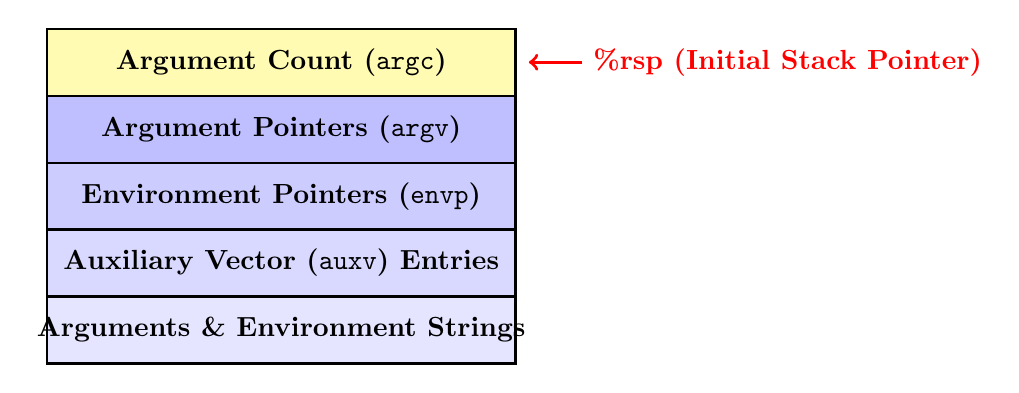
\begin{tikzpicture}[scale=0.85]
    \draw[thick, fill=blue!10] (0, 0) rectangle (7, 1) node[pos=.5] {\textbf{Arguments \& Environment Strings}};
    \draw[thick, fill=blue!15] (0, 1) rectangle (7, 2) node[pos=.5] {\textbf{Auxiliary Vector (\texttt{auxv}) Entries}};
    \draw[thick, fill=blue!20] (0, 2) rectangle (7, 3) node[pos=.5] {\textbf{Environment Pointers (\texttt{envp})}};
    \draw[thick, fill=blue!25] (0, 3) rectangle (7, 4) node[pos=.5] {\textbf{Argument Pointers (\texttt{argv})}};
    \draw[thick, fill=yellow!30] (0, 4) rectangle (7, 5) node[pos=.5] {\textbf{Argument Count (\texttt{argc})}};
    \draw[->, very thick, red] (8, 4.5) -- (7.2, 4.5) node[right, pos=0, red] {\textbf{\%rsp (Initial Stack Pointer)}};
\end{tikzpicture}
\caption{System V AMD64 Initial Process Stack Layout.}
\label{fig:user_stack_layout}
\end{figure}

The auxiliary vector communicates runtime information from the kernel to the dynamic linker:
\begin{itemize}
    \item \texttt{AT\_PHDR}: Virtual base address of the Program Header Table;
    \item \texttt{AT\_PHNUM}: Number of program header entries;
    \item \texttt{AT\_ENTRY}: Executable entry point;
    \item \texttt{AT\_PAGESZ}: System hardware page size (4096 bytes);
    \item \texttt{AT\_RANDOM}: 16 bytes of cryptographically secure random values (for stack canaries).
\end{itemize}

% ==============================================================================
\section{Summary}
\label{sec:summary_chap2}
% ==============================================================================

Processes and threads are the core abstractions of concurrent operating systems. A process provides an isolated virtual address space and kernel resources, while threads provide concurrent execution contexts sharing that memory. 

To prevent race conditions, critical regions must be protected through mutual exclusion primitives, ranging from atomic hardware instructions (\texttt{lock cmpxchg}) to user-space futexes. Hydra coordinates execution through a priority-aware preemptive scheduler running at 100~Hz with dynamic starvation prevention, executing context switches by saving complete \texttt{TaskRegisters} and manipulating x86\_64 \texttt{CR3} and \texttt{FS\_BASE} registers. Finally, synchronous rendezvous IPC provides mathematically failure-isolated communication across Ring~3 system servers.

% ==============================================================================
\section{Exercises and Review Problems}
\label{sec:exercises_chap2}
% ==============================================================================

\begin{enumerate}
    \item \textbf{Process vs. Thread:} What state is shared between multiple threads executing within the same process? What state must remain strictly private to each thread?
    \item \textbf{Context Switch Mechanics:} During an x86\_64 interrupt, which registers are pushed onto the stack automatically by the CPU hardware, and which registers must be preserved by the operating system software stub?
    \item \textbf{Address Space Invalidation:} Why does writing a new physical address into \texttt{CR3} degrade subsequent memory access performance for a few hundred CPU cycles? How do modern processors mitigate this penalty?
    \item \textbf{Race Conditions:} Write a short pseudo-code snippet illustrating how two threads concurrently executing \texttt{counter = counter + 1} can lose an update if preempted at the machine instruction level.
    \item \textbf{Peterson's Algorithm:} Explain how Peterson's two-process mutual exclusion algorithm functions. Why does it fail on modern multi-core x86\_64 processors unless hardware memory fences (\texttt{mfence}) are inserted?
    \item \textbf{Futex Efficiency:} Why are Linux-compatible futexes dramatically faster than traditional UNIX semaphore system calls in the uncontended locking case?
    \item \textbf{Starvation Prevention:} In Hydra's scheduler, how does the \texttt{STARVATION\_LIMIT} parameter ensure that low-priority batch threads eventually make progress even in the presence of continuous high-priority network traffic?
    \item \textbf{Deadlock Analysis:} State the four necessary conditions for deadlock (Coffman conditions). Which condition is broken by Dijkstra's resource ordering solution to the Dining Philosophers Problem?
    \item \textbf{CPU Power Management:} What does the assembly instruction \texttt{hlt} do? Why is it vital that interrupts be re-enabled (\texttt{sti}) immediately prior to halting the CPU inside the idle task loop?
    \item \textbf{Design Problem:} Design an asynchronous message-passing IPC system with bounded mailboxes. What happens when a mailbox becomes full? How does your design compare to Hydra's synchronous rendezvous model in terms of memory footprint and susceptibility to denial-of-service attacks?
\end{enumerate}
